% File: queue-perm-direct.tex

\documentclass{standalone}

\usepackage{tikz}
\usetikzlibrary{shapes, arrows.meta, positioning}

\begin{document}
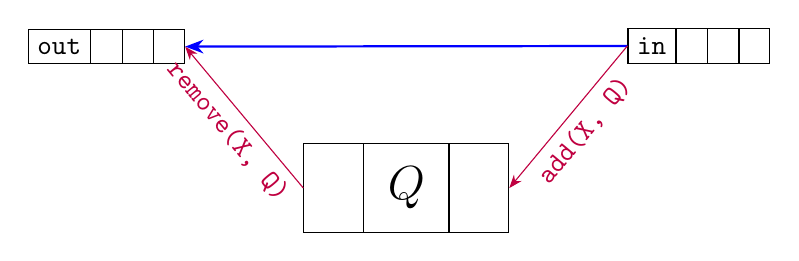
\begin{tikzpicture}[seq/.style = {rectangle split, 
  rectangle split horizontal, 
  rectangle split draw splits = true, 
  rectangle split parts = 4,
  draw}]

  \node[draw, rectangle split,
	rectangle split horizontal, 
  	rectangle split parts = 3,
	inner sep = 3mm
      ] (queue) {\nodepart{two} {\LARGE $Q$}};

  \node[seq, above right = 1.0cm and 1.5cm of queue] (in) {\texttt{in}};
  \node[seq, above left = 1.0cm and 1.5cm of queue] (out) {\texttt{out}};

  \draw[->, >=Stealth, thick, blue] (in) to (out);

  \draw[->, >=Stealth, purple] (in.west) to node[sloped, below] {\texttt{add(X, Q)}} (queue.east);
  \draw[->, >=Stealth, purple] (queue.west) to node[sloped, below] {\texttt{remove(X, Q)}} (out.east);
\end{tikzpicture}
\end{document}
